% =====================================================================
%  Chapter 3 -- Hybrid Zero Dynamics Gait Synthesis for RABBIT
%  IEEE conference format (IEEEtran).
%
%  Compile with:  pdflatex ch3_ieee_report.tex   (run twice for refs)
%
%  Every numerical value in this report is a MEASURED quantity taken from
%  the Chapter 3 implementation in this repository, not a literature value.
%  Sources are named in the text so each can be re-derived.
% =====================================================================
\documentclass[10pt,conference]{IEEEtran}

\usepackage[T1]{fontenc}
\usepackage{amsmath,amssymb}
\usepackage{booktabs}
\usepackage{graphicx}
\graphicspath{{figures/}}
\usepackage{url}

\interdisplaylinepenalty=2500

\begin{document}

\title{Hybrid Zero Dynamics Gait Synthesis for the RABBIT Biped:\\
Transcription Accuracy, Stability Certification,\\
and the Cost of a Minimum-Norm Controller}

\author{\IEEEauthorblockN{Malek Mohammad}
\IEEEauthorblockA{RABBIT Bipedal Robot Project\\
Chapter 3: Hybrid Walking Pipeline\\
Email: malek.mohammad132@gmail.com}}

\maketitle

\begin{abstract}
This report documents a complete implementation of hybrid zero dynamics (HZD)
gait synthesis for the RABBIT planar biped, covering the hybrid model, virtual
constraints, input--output linearization, direct-collocation trajectory
optimization, and four control laws. Three findings are reported that are not
predicted by the standard treatment. First, the Hermite--Simpson transcription
loses its formal order of accuracy not through any error in the transcription
itself---the median defect converges at order $5.1$--$5.9$, exactly as
theory requires---but through the \emph{smoothness of the output basis}: a
degree-3 clamped B-spline is only $C^2$ at its interior knots, and the two
resulting kinks in the closed-loop vector field cap $\max|\text{defect}|$ at
order ${\approx}1.5$, a $4300\times$ loss in transcription accuracy against a
smoother basis. Second, the restricted Poincar\'e map computed by quadrature
over the Bezier coefficients alone agrees with a 26-simulation Poincar\'e
estimate to five digits ($\delta^2_{\mathrm{zero}}=0.75988$ versus
$\rho=0.75989$), certifying orbital stability at roughly $1/80$ the cost of one
constraint gradient. Third, and counter-intuitively, the \emph{unconstrained}
CLF-QP is the worst of the three control laws tested: by requesting the
least-norm input that satisfies the RES-CLF rate, it discards precisely the
surplus convergence that was paying for stability across the impact map, and
the demanded torque nearly doubles. The reference gait is periodic
($8.1\times10^{-7}$), mesh-verified, and orbitally stable ($\rho = 0.760$),
but fails the NEC3 impulse-friction condition at $|I_x|/I_z = 2.44$ against
$\mu_s = 0.4$---a failure invisible to the continuous-phase friction margin.
\end{abstract}

\begin{IEEEkeywords}
Bipedal locomotion, hybrid zero dynamics, virtual constraints, direct
collocation, control Lyapunov functions, orbital stability.
\end{IEEEkeywords}

% =====================================================================
\section{Introduction}
% =====================================================================

RABBIT is a five-link planar bipedal robot with point feet,
built as a testbed for underactuated walking control~\cite{chevallereau2003}.
Because the feet are points, the robot is underactuated during single support:
four actuators must regulate a seven-degree-of-freedom system. The hybrid zero
dynamics (HZD) framework of Westervelt \emph{et al.}~\cite{westervelt2007}
resolves this by imposing four \emph{virtual constraints}---output functions
driven to zero by feedback---which reduce the closed-loop behaviour to a
low-dimensional invariant surface whose stability can be analysed directly.

This report documents an implementation of that framework as a complete,
verified pipeline, and reports what was measured when the theory met a
specific robot. The emphasis throughout is on quantities that were
\emph{measured rather than assumed}: where the implementation and the standard
treatment disagree, the disagreement is reported with the number that produced
it.

The contributions are:

\begin{enumerate}
\item An analysis (Section~\ref{sec:order}) localizing a loss of transcription
      accuracy to the smoothness of the output basis rather than to the
      collocation scheme, with the mechanism confirmed by four independent
      measurements.
\item A closed-form orbital stability certificate (Section~\ref{sec:hzd})
      validated against forward simulation to five digits.
\item A measured comparison of four control laws under a binding torque limit
      (Section~\ref{sec:control}) showing that minimum-norm optimality is
      actively harmful across a hybrid impact.
\item A characterization (Section~\ref{sec:nec3}) of the one constraint in the
      \S6.3.4 set that a coarse mesh evaluates incorrectly while still passing
      mesh verification.
\end{enumerate}

% =====================================================================
\section{Robot Model and Hybrid Dynamics}
% =====================================================================

The robot is modelled as a hybrid system alternating a continuous single-support
phase with an instantaneous double-support impact.

\subsection{Continuous phase}

During single support the stance foot is pinned, giving a holonomic constraint
$P_{\mathrm{st}}(q) = \text{const}$. Differentiating twice yields
$J_{\mathrm{st}}\ddot q + \dot J_{\mathrm{st}}\dot q = 0$, and with the contact
wrench $\lambda$ as multiplier the constrained dynamics are the KKT system
%
\begin{equation}
\begin{bmatrix} M(q) & -J_{\mathrm{st}}^\top \\ J_{\mathrm{st}} & 0 \end{bmatrix}
\begin{bmatrix} \ddot q \\ \lambda \end{bmatrix}
=
\begin{bmatrix} Bu - V(q,\dot q) - G(q) \\ -\dot J_{\mathrm{st}}\dot q \end{bmatrix}.
\label{eq:kkt}
\end{equation}
%
The left-hand matrix is independent of $u$, so a single factorization with five
right-hand sides (one drift, four input directions) recovers the entire
control-affine structure \emph{exactly}, with no finite differencing:
%
\begin{equation}
\ddot q = \ddot q_{\mathrm{drift}} + \ddot q_{\mathrm{in}} u, \qquad
\lambda = \lambda_{\mathrm{drift}} + \lambda_{\mathrm{in}} u,
\end{equation}
%
and therefore $\dot x = f(x) + g(x)u$ with
$f = [\dot q;\ \ddot q_{\mathrm{drift}}]$ and
$g = [0;\ \ddot q_{\mathrm{in}}]$. That the ground reaction force is
\emph{affine in $u$} is what later permits the friction cone to be written as a
linear inequality inside a quadratic program (Section~\ref{sec:control}).

\subsection{Impact and the hybrid model}

The guard $S = \{x : h_{\mathrm{sw}}(q) = 0,\ \dot h_{\mathrm{sw}} < 0\}$ fires
when the swing foot strikes with downward velocity. The reset $\Delta$ applies a
rigid impulsive impact enforcing $J_{\mathrm{sw}}\dot q^+ = 0$ (the new stance
foot does not rebound or slip), followed by a coordinate relabelling that swaps
the legs. The relabelling is an involution, verified to machine precision.
Dimensions are summarized in Table~\ref{tab:dims}.

\begin{table}[t]
\caption{Model dimensions and phase parametrization}
\label{tab:dims}
\centering
\begin{tabular}{lc}
\toprule
Quantity & Value \\
\midrule
Generalized coordinates $n_q$        & 7 \\
Full state dimension $n_x$           & 14 \\
Actuators $n_u$                      & 4 \\
Outputs $n_y$                        & 4 \\
Actuated coordinates                 & $q_4 \ldots q_7$ \\
Phase variable $\theta = c^\top q$   & $c = [0\,0\,1\,1\,0.5\,0\,0]$ \\
Phase range $[\theta^-,\theta^+]$    & $[-0.15,\ 0.30]$ rad \\
Collocation nodes $N$                & 41 \\
\bottomrule
\end{tabular}
\end{table}

% =====================================================================
\section{Virtual Constraints and Input--Output Linearization}
% =====================================================================

\subsection{The phase variable}

Rather than indexing the desired motion by time, the outputs are indexed by the
absolute stance leg angle
%
\begin{equation}
\theta = q_T + q_{LA}^{\mathrm{st}} = c^\top q, \qquad
s = \frac{\theta - \theta^-}{\theta^+ - \theta^-},
\end{equation}
%
so $s$ runs $0 \to 1$ across a step. This makes the gait \emph{self-paced}: the
robot's own configuration reports how far through the step it is, and the
resulting feedback is time-invariant. Two properties are used throughout: $c$ is
constant, so $\partial s/\partial q$ carries no state dependence and $L_f^2 y$
acquires only a single curvature term; and $\theta$ cannot wrap, so the
optimizer never encounters a phantom discontinuity.

\subsection{Outputs and relative degree}

With $y = y_0(q) - y_d(s(q),\alpha)$, the outputs have uniform relative degree
two---$u$ does not appear in $\dot y$---so
%
\begin{equation}
\ddot y = L_f^2 y(x) + L_g L_f y(x)\, u,
\end{equation}
%
where, substituting the affine split from \eqref{eq:kkt},
%
\begin{align}
L_f^2 y &= J_y\, \ddot q_{\mathrm{drift}} - \tfrac{\partial^2 y_d}{\partial s^2}\dot s^2, \\
L_g L_f y &= J_y\, \ddot q_{\mathrm{in}}.
\end{align}
%
Both are exact. Where the decoupling matrix $L_gL_fy$ is invertible,
%
\begin{equation}
u = u_{\mathrm{ff}}(x) + (L_gL_fy)^{-1}\mu, \quad
u_{\mathrm{ff}} = -(L_gL_fy)^{-1}L_f^2 y,
\label{eq:iolin}
\end{equation}
%
yields the double integrator $\ddot y = \mu$. Every control law in this report
differs \emph{only} in how it selects $\mu$.

\subsection{Profile evaluation and boundary handling}

Two implementation details of $y_d$ affect accuracy downstream and are shown in
Fig.~\ref{fig:yd}. First, a step that fails to strike can drive $s$ far outside
$[0,1]$, where an unclamped polynomial extrapolates without bound, so $s$ is
clamped---but with a margin, engaging outside $[-0.5, 1.5]$ rather than at the
endpoints. Clamping hard at exactly $[0,1]$ is a trap: $s = 0$ begins every
step and floating point places it on either side, so a hard clamp intermittently
zeroes $\partial s/\partial q$, which zeroes $\dot s$, which silently drops the
$(\partial y_d/\partial s)\dot s$ term from $\dot y$. The symptom is a gait that
appears to start off the zero dynamics surface even when constructed to start on
it. Critically, wherever the clamp does engage the reported derivative must be
set to zero to match the frozen value; returning the frozen boundary slope
instead hands the caller a $\partial y_d/\partial s$ that is not the derivative
of the $y_d$ it accompanies, and $J_y = H - (\partial y_d/\partial s)\,
\partial s/\partial q$ then acquires a term that should not be there.

Second, the B-spline path has no analytic second derivative available, so
$\partial^2 y_d/\partial s^2$ is obtained by central differencing the analytic
first derivative. The stencil is kept entirely inside $[0,1]$ rather than
clipped against the endpoint: clipping silently degrades the formula to
one-sided, dropping it from $O(h^2)$ to $O(h)$ and costing five orders of
accuracy at $s=1$---measured $1.76\times10^{-4}$ there against
$4\times10^{-9}$ in the interior. That endpoint is touchdown on every step, and
it is where $|\partial^2 y_d/\partial s^2|$ is largest, so the error feeds
straight into $L_f^2y$ at the worst moment.

\begin{figure*}[t]
\centering
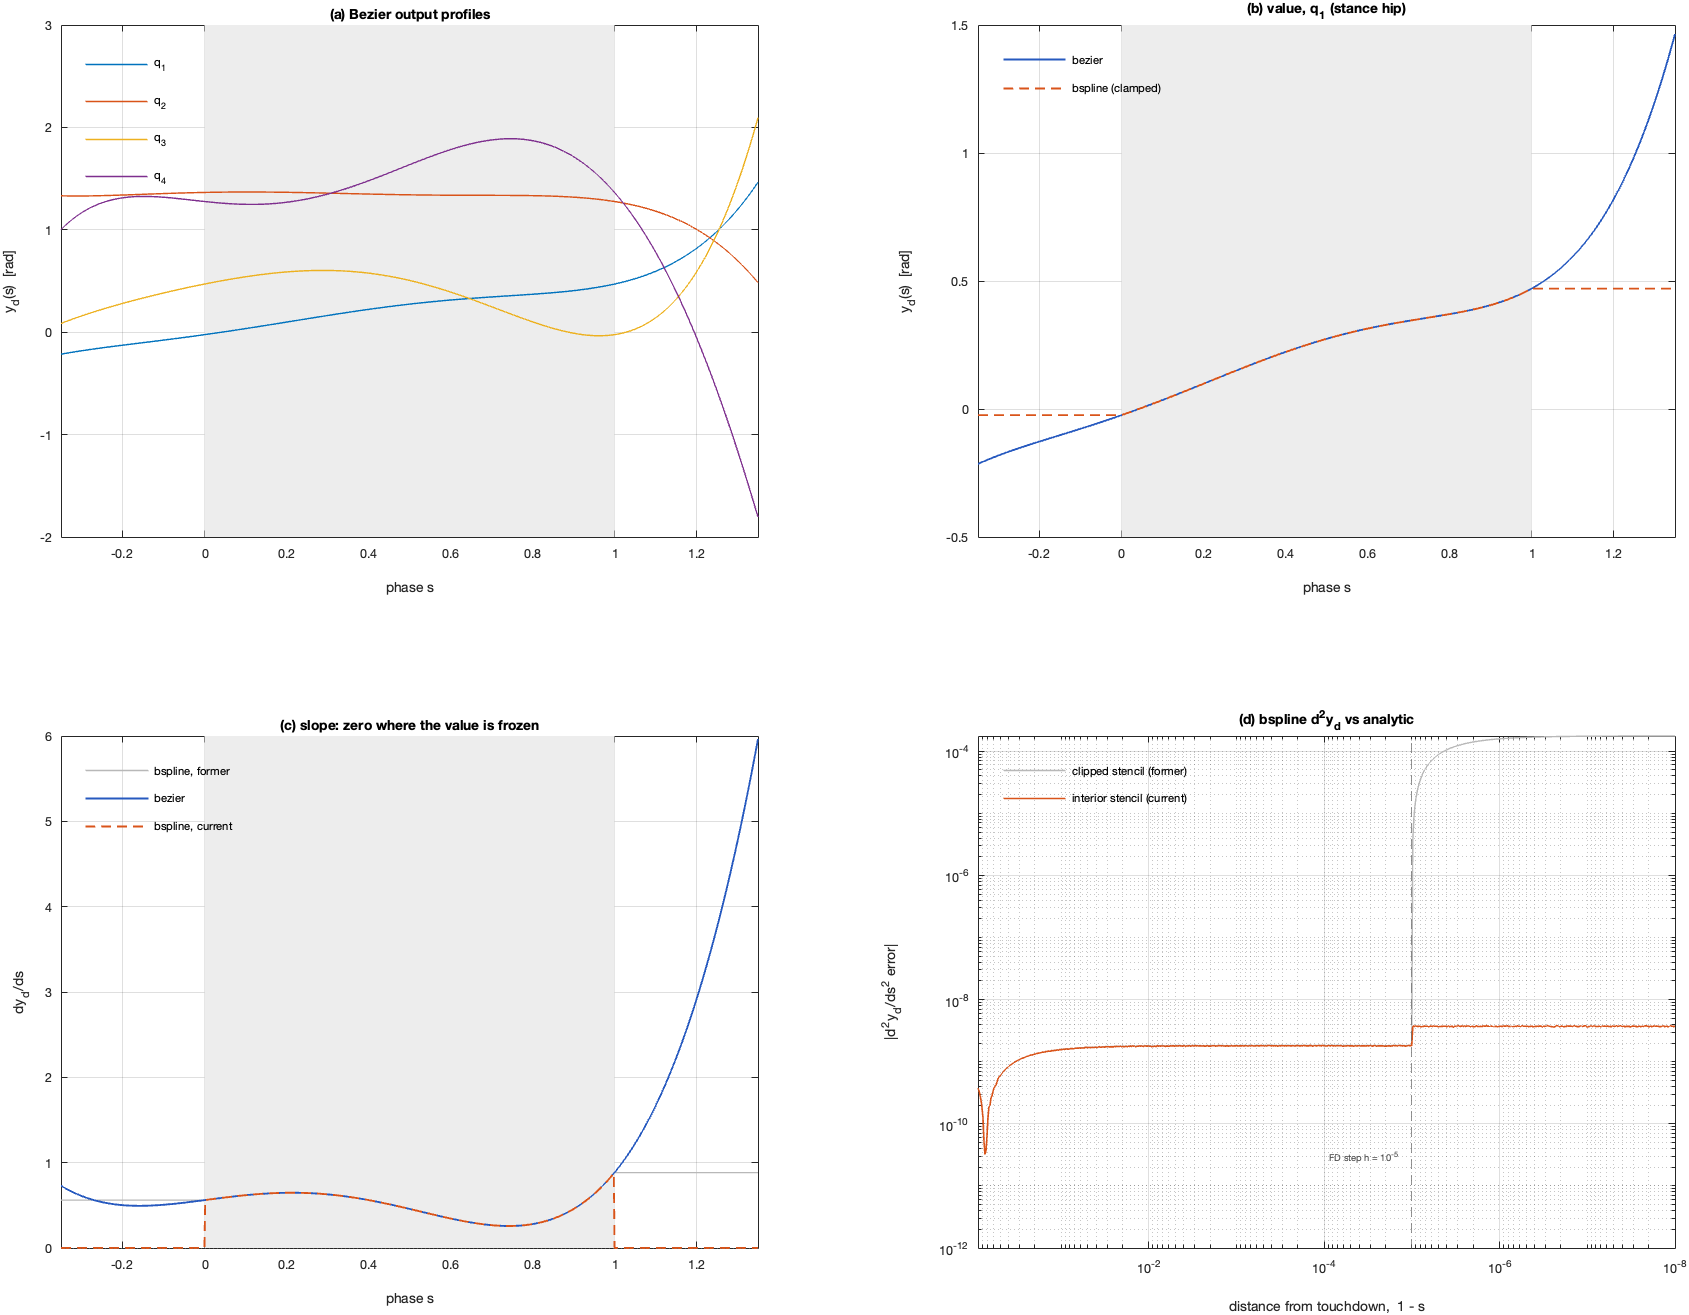
\includegraphics[width=0.94\textwidth]{fig_yd_smoothness.png}
\caption{Evaluation of the desired output profile. \textbf{(a)} The four Bezier
output profiles over the step; the shaded band is $s \in [0,1]$. \textbf{(b)}
Value of the stance-hip profile, Bezier versus clamped B-spline: outside
$[0,1]$ the clamped spline freezes while the polynomial continues.
\textbf{(c)} The corresponding slope. The current implementation (dashed)
reports zero derivative wherever the value is frozen, matching the curve it
accompanies; the former behaviour (grey) returned the frozen boundary slope
instead. \textbf{(d)} Error in the central-differenced
$\partial^2 y_d/\partial s^2$ as touchdown is approached. Holding the stencil
inside the domain (orange) keeps the error near $2\times10^{-9}$ all the way to
$s = 1$; the clipped stencil (grey) degrades to $O(h)$ and rises by roughly
five orders of magnitude within the finite-difference step of the endpoint.}
\label{fig:yd}
\end{figure*}

Conditioning of $L_gL_fy$ was characterized empirically. Over the reference gait
$\mathrm{rcond}$ remains in $[5.6\times10^{-3},\ 8.3\times10^{-3}]$; across
$20\,000$ random states spanning the full $\pm\pi$ joint box the worst value is
$8.0\times10^{-6}$. Contrary to the common intuition that knee extension drives
singularity, a $121\times121$ grid over both knees bottoms out at
$2.1\times10^{-7}$ at deep double \emph{flexion}, not at lock. What actually
degrades conditioning is the \emph{profile slope}: $\partial y_d/\partial s$
enters $J_y$ directly, and stretching $\alpha$ about $\alpha_0$ by $100\times$
degrades $\mathrm{rcond}$ from $5.8\times10^{-3}$ to $1.0\times10^{-4}$.

% =====================================================================
\section{Direct Collocation Gait Synthesis}
% =====================================================================

\subsection{Transcription}

The gait is found by direct collocation with a Hermite--Simpson transcription.
For each interval, with $h = T/(N-1)$,
%
\begin{align}
x_m &= \tfrac{1}{2}(x_k + x_{k+1}) + \tfrac{h}{8}\left(f_k - f_{k+1}\right), \label{eq:hsmid}\\
\zeta_k &= x_{k+1} - x_k - \tfrac{h}{6}\left(f_k + 4f_m + f_{k+1}\right), \label{eq:hsdef}
\end{align}
%
where $\zeta_k$ is the defect. Driving $\zeta \to 0$ \emph{is} the dynamics
constraint: no ODE solver appears anywhere inside the optimizer loop. Two
consequences matter. The stance foot is pinned at every node rather than merely
integrated, so contact cannot drift during a step; and the same Simpson weights
that define the defects also integrate the cost, so cost and dynamics share one
consistent quadrature.

Inside the solve the input is the feedforward \eqref{eq:iolin} alone. This is
deliberate: the transcription pins $y = \dot y = 0$ at node~1, and
$u_{\mathrm{ff}}$ renders that surface invariant, so any feedback term would
multiply zero while adding nonlinearity for the optimizer to differentiate
through. It also makes the reported cost honest---the torque being integrated is
the torque the gait requires, not a tracking transient.

\subsection{Seeding and continuation}

The initial guess is produced by rolling out the seed gait under pure
feedforward and sampling nodes from the resulting trajectory via the
integrator's dense output. This lands the guess on the zero dynamics surface to
$4.1\times10^{-7}$ and satisfies the defects to integration accuracy from the
first evaluation; only periodicity and the walking-rate condition remain
genuinely violated, which is a far better starting point than interpolating
between poses.

Requirements are not imposed all at once. Box and band constraints on speed,
posture and impulse are reached by \emph{marching}: a ladder of intermediate
targets, each solve warm-started from the last converged result. The measured
justification is stark. One posture rung started from a cold solve cost 3.1
hours across three solves and still missed the verification tolerance by
$1.5\times$; the same rung started from a converged, verified gait and moving
one bound slightly is the regime sequential quadratic programming handles well.

% =====================================================================
\section{The \S6.3.4 Constraint Set}
\label{sec:constraints}
% =====================================================================

The full constraint set of~\cite[\S6.3.4]{westervelt2007} is implemented as 17
individually gated rows (Table~\ref{tab:constraints}).

\begin{table}[t]
\caption{Implemented \S6.3.4 constraints}
\label{tab:constraints}
\centering
\begin{tabular}{llc}
\toprule
Constraint & Gate & Source \\
\midrule
Friction cone $|F_x| \le \mu_s F_z$      & \texttt{friction}    & NIC1 \\
Minimum normal force $F_z \ge F_z^{\min}$& \texttt{grf}         & NIC2 \\
Swing clearance; transversal strike      & \texttt{swing\_clear}& NIC3 \\
Average walking rate                     & \texttt{enforce\_nec1} & NEC1 \\
Post-impact swing-leg lift-off           & \texttt{liftoff}     & NEC2 \\
Impulse compressive; inside cone         & \texttt{impact}      & NEC3 \\
Fixed point exists; is stable            & \texttt{hzd}         & NEC4/5 \\
$\theta$ strictly monotonic              & \texttt{phase\_mono} & HH6 \\
Decoupling matrix invertible on $Z$      & \texttt{decoupling}  & HH2 \\
\bottomrule
\end{tabular}
\end{table}

Two implementation points are worth recording. First, hybrid invariance
(HH4/HH5, $\Delta(S \cap Z) \subset Z$) receives \emph{no row}. This
transcription pins $y = \dot y = 0$ at node~1 and equates $\Delta(x_N)$ to
node~1, so invariance is \emph{implied}; adding it explicitly would duplicate
rows the periodicity block already spans and introduce rank deficiency. It is
therefore measured rather than assumed, at $3.9\times10^{-6}$ on the reference
gait. Second, the ordering in which gates are enabled matters: GRF must precede
friction, because friction is $|F_x|/F_z$ and enabling it while $F_z$ still
crosses zero sets the optimizer chasing a division by zero. The full working
order is \texttt{grf} $\to$ \texttt{friction} $\to$ torque $\to$ impulse $\to$
the cheap geometric gates $\to$ \texttt{liftoff} $\to$ \texttt{impact}.

% =====================================================================
\section{Transcription Accuracy and Basis Smoothness}
\label{sec:order}
% =====================================================================

\begin{figure*}[t]
\centering
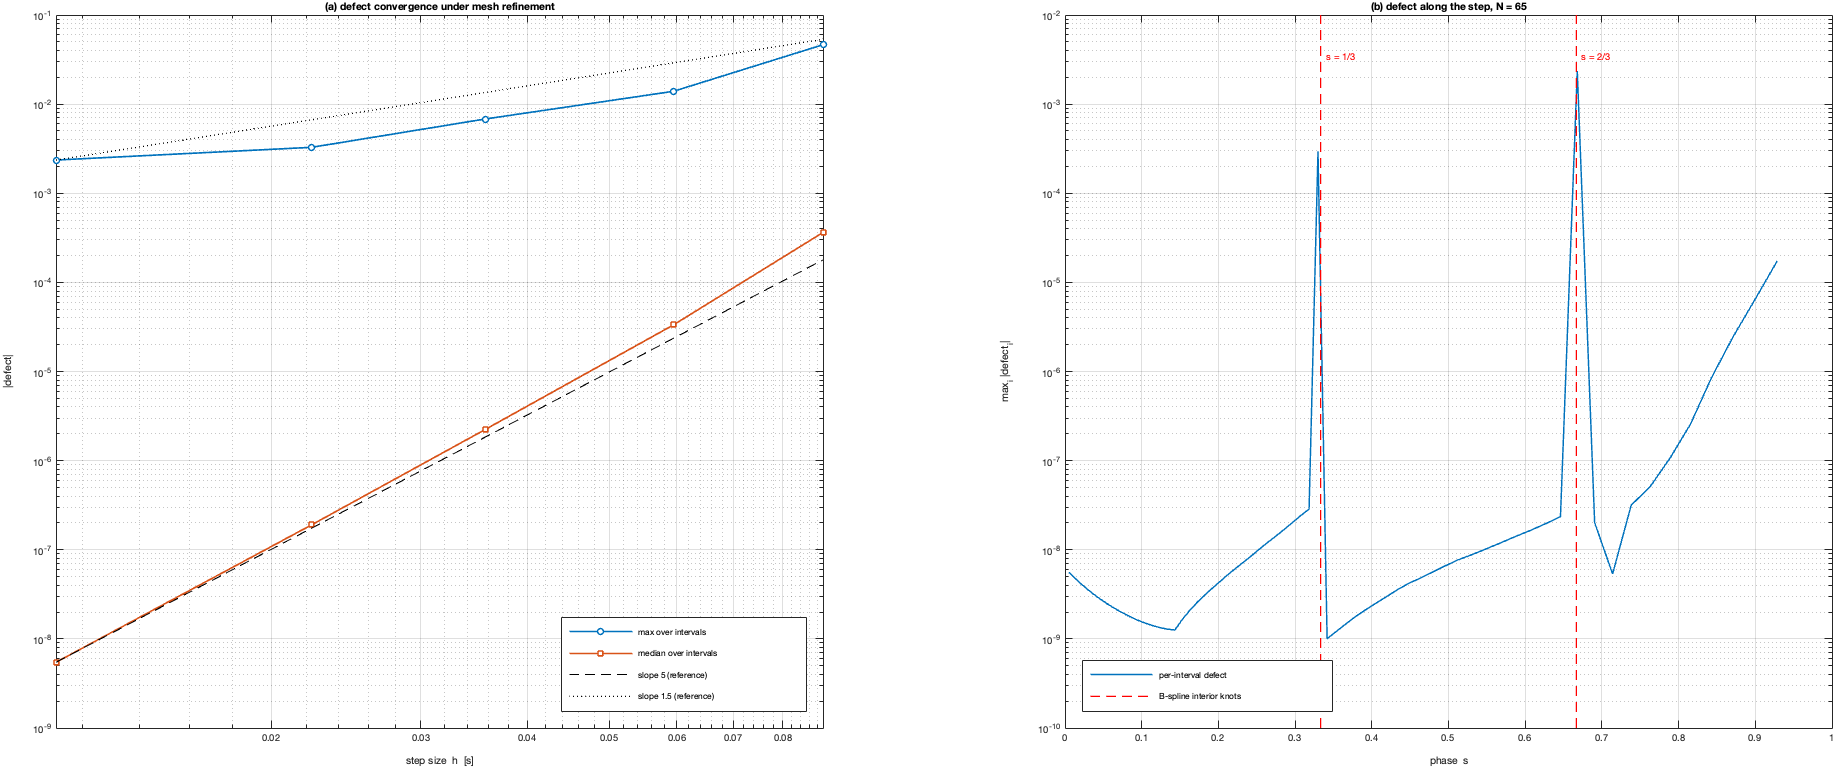
\includegraphics[width=\textwidth]{fig_ch3_defect_order.png}
\caption{Hermite--Simpson defect of the seed rollout. \textbf{(a)} Under mesh
refinement the \emph{median} defect over intervals tracks the reference slope~5
almost exactly---the $O(h^5)$ local truncation error the scheme is required to
have---while the \emph{maximum} tracks slope~1.5. The two statistics diverge by
six orders of magnitude at the finest mesh, which is what identifies the loss as
localized rather than global. \textbf{(b)} The per-interval defect along one
step at $N=65$, plotted against phase $s$. Two spikes, three to four orders of
magnitude above the surrounding baseline, land on the interior knots of the
degree-3 clamped B-spline at $s=1/3$ and $s=2/3$ (dashed), where $y_d$ is $C^2$
and no smoother. Every interval away from a knot converges at the design rate.}
\label{fig:order}
\end{figure*}

Hermite--Simpson is a fourth-order scheme; the residual \eqref{eq:hsdef} has
local truncation error $O(h^5)$. Refining the mesh and observing the defect is
the sharpest available check that the transcription is correctly implemented, so
it is asserted in the verification suite. On the shipped configuration that
assertion \emph{fails}, at observed order ${\approx}1.5$. This section
establishes that the transcription is nevertheless correct, and localizes the
cause.

\subsection{Measurement}

Table~\ref{tab:order} reports the seed-rollout defect under mesh refinement.
Two statistics are shown: the maximum over all intervals and states, which is
what the assertion tests, and the median over intervals.

\begin{table}[t]
\caption{Defect convergence of the seed rollout}
\label{tab:order}
\centering
\begin{tabular}{ccccc}
\toprule
$N$ & $h$ [s] & $\max|\zeta|$ & order & median order \\
\midrule
9  & 0.0892 & $4.639\times10^{-2}$ & ---   & ---  \\
13 & 0.0595 & $1.393\times10^{-2}$ & 2.97 & 5.89 \\
21 & 0.0357 & $6.804\times10^{-3}$ & 1.40 & 5.29 \\
33 & 0.0223 & $3.276\times10^{-3}$ & 1.56 & 5.23 \\
65 & 0.0112 & $2.358\times10^{-3}$ & 0.47 & 5.12 \\
\bottomrule
\end{tabular}
\end{table}

The median defect converges at order $5.1$--$5.9$, which is precisely the
$O(h^5)$ the raw residual should exhibit. \textbf{The transcription is correct.}
What fails is the maximum, which is dominated by two or three isolated
intervals. Fig.~\ref{fig:order}(a) shows the two statistics separating by six
orders of magnitude as the mesh is refined.

\subsection{Localization}

Four independent measurements identify the same two instants:

\begin{enumerate}
\item The maximum always occurs in state row 14 ($\dot q_7$, the swing-knee
      velocity), at $t/T \approx 0.52$ and $0.84$, at \emph{every} mesh
      resolution---i.e.\ at fixed physical times, not fixed indices.
\item Converting those times to phase gives $s \approx 0.3333$ and
      $s \approx 0.6667$.
\item The adaptive integrator used to build the seed independently collapses its
      step size at the same instants, from a $5\times10^{-3}$ ceiling to
      $8.3\times10^{-5}$ at $t/T = 0.512$, $0.833$--$0.836$.
\item Tightening the integrator tolerance from $10^{-8}$ to $10^{-12}$ changes
      $\max|\zeta|$ by $0.04\%$, ruling out integration error.
\end{enumerate}

The default output basis is a clamped B-spline of degree 3 with six control
points. Its knot vector is
$[0,0,0,0,\ \tfrac13,\ \tfrac23,\ 1,1,1,1]$---interior knots at exactly
$1/3$ and $2/3$, matching the measured kink locations. Fig.~\ref{fig:order}(b)
plots the defect against phase directly: the two spikes sit on the knots, and
every interval away from them converges at the design rate. At a simple interior
knot a degree-$p$ spline is $C^{p-1}$, so $y_d$ is $C^2$ and no smoother. The second
derivative $\partial^2 y_d/\partial s^2$ therefore has a corner, which
propagates through $L_f^2y$ into $u_{\mathrm{ff}}$ and hence into $\ddot q$,
leaving the state trajectory $C^2$ but not $C^3$. Hermite--Simpson requires
more smoothness than that to achieve $O(h^5)$, so exactly the intervals
straddling the knots lose order while all others retain it.

The knot smoothness is the dominant effect, but it is not the only one: on this
path $\partial^2 y_d/\partial s^2$ is itself central-differenced rather than
analytic (Fig.~\ref{fig:yd}(d)), so a further $O(h_{\mathrm{FD}}^2)$ error
enters $L_f^2 y$. Both are properties of the \emph{basis}, not of the
collocation scheme, which is the point of this section.

\subsection{Consequence}

The effect is not marginal (Table~\ref{tab:basis}).

\begin{table}[t]
\caption{Transcription accuracy versus output basis, $N=49$}
\label{tab:basis}
\centering
\begin{tabular}{lcc}
\toprule
Basis & Order & $\max|\zeta|$ \\
\midrule
B-spline, degree 3 (default) & 1.61 & $1.675\times10^{-3}$ \\
B-spline, degree 5           & 4.51 & $3.874\times10^{-7}$ \\
Bezier                       & 4.51 & $3.874\times10^{-7}$ \\
\bottomrule
\end{tabular}
\end{table}

A smoother basis buys roughly $4300\times$ in transcription accuracy at no
modelling cost. The degree-3 default is retained deliberately, as a genuinely
different curve from the Bezier form and hence an independent cross-check of the
basis-agnostic pipeline; the order assertion is left failing as an honest
report of the trade-off rather than tuned away. The practical guidance is that
any gait intended for quantitative use should be solved on the smoother basis.

The broader methodological point is that a mesh-refinement study is a test of
the \emph{whole} discretization---scheme \emph{and} the smoothness of everything
the scheme differentiates. Reporting only $\max|\zeta|$ would have indicted the
collocation code; the median statistic is what separates the two hypotheses.

% =====================================================================
\section{Stability Certification via the Zero Dynamics}
\label{sec:hzd}
% =====================================================================

Periodicity is not stability. The periodicity equality makes the start state a
\emph{fixed point} of the step-to-step map, and a fixed point can repel, no
matter how small the periodicity residual.

Two independent certificates are computed. The direct one perturbs the state and
integrates, forming the Poincar\'e map Jacobian numerically and returning its
spectral radius $\rho$; it costs 26 step simulations. The indirect one reduces
the dynamics on $Z$ to a scalar second-order ODE
%
\begin{equation}
a(\theta)\ddot\theta + b(\theta)\dot\theta^2 + c(\theta) = 0
\end{equation}
%
by projecting onto the covector $w$ that annihilates \emph{both} the actuators
and the contact wrench ($wB = 0$, $wJ_{\mathrm{st}}^\top = 0$). An integrating
factor $m = \exp\!\int b/a$ and the substitution $\sigma = m\dot\theta$ convert
this to the $(\kappa_1,\kappa_2)$ form of~\cite{westervelt2007}, in which the
step map is \emph{affine} in $\zeta = \sigma^2/2$, so its fixed point and
eigenvalue $\delta^2_{\mathrm{zero}}$ are closed form.

The two agree to five digits:
%
\begin{equation}
\delta^2_{\mathrm{zero}} = 0.75988, \qquad \rho = 0.75989 .
\end{equation}
%
The reduction is validated against the full 14-state model to
$7.8\times10^{-10}$, and the invariant $\tfrac12\sigma^2 + V_{\mathrm{zero}}(\theta)$
is conserved along a genuine rollout to $8.7\times10^{-7}$---a quantity that
cannot hold by accident if the integrating factor is wrong.

The certificate is thus available from $\alpha$ alone, by one quadrature, with
no simulation. It is nonetheless disabled by default as a \emph{constraint}: one
constraint evaluation rises from $0.003$~s to $0.241$~s, so one finite-difference
gradient rises from ${\approx}1$~s to ${\approx}77$~s. Because this
transcription imposes periodicity directly, a converged solve is already at a
fixed point, making NEC4/NEC5 a \emph{check} on the fixed point found rather
than the mechanism for finding one. The book requires them as constraints
because its optimization parametrizes $\alpha$ alone and never propagates a
state.

% =====================================================================
\section{Reference Gait}
% =====================================================================

\begin{figure*}[t]
\centering
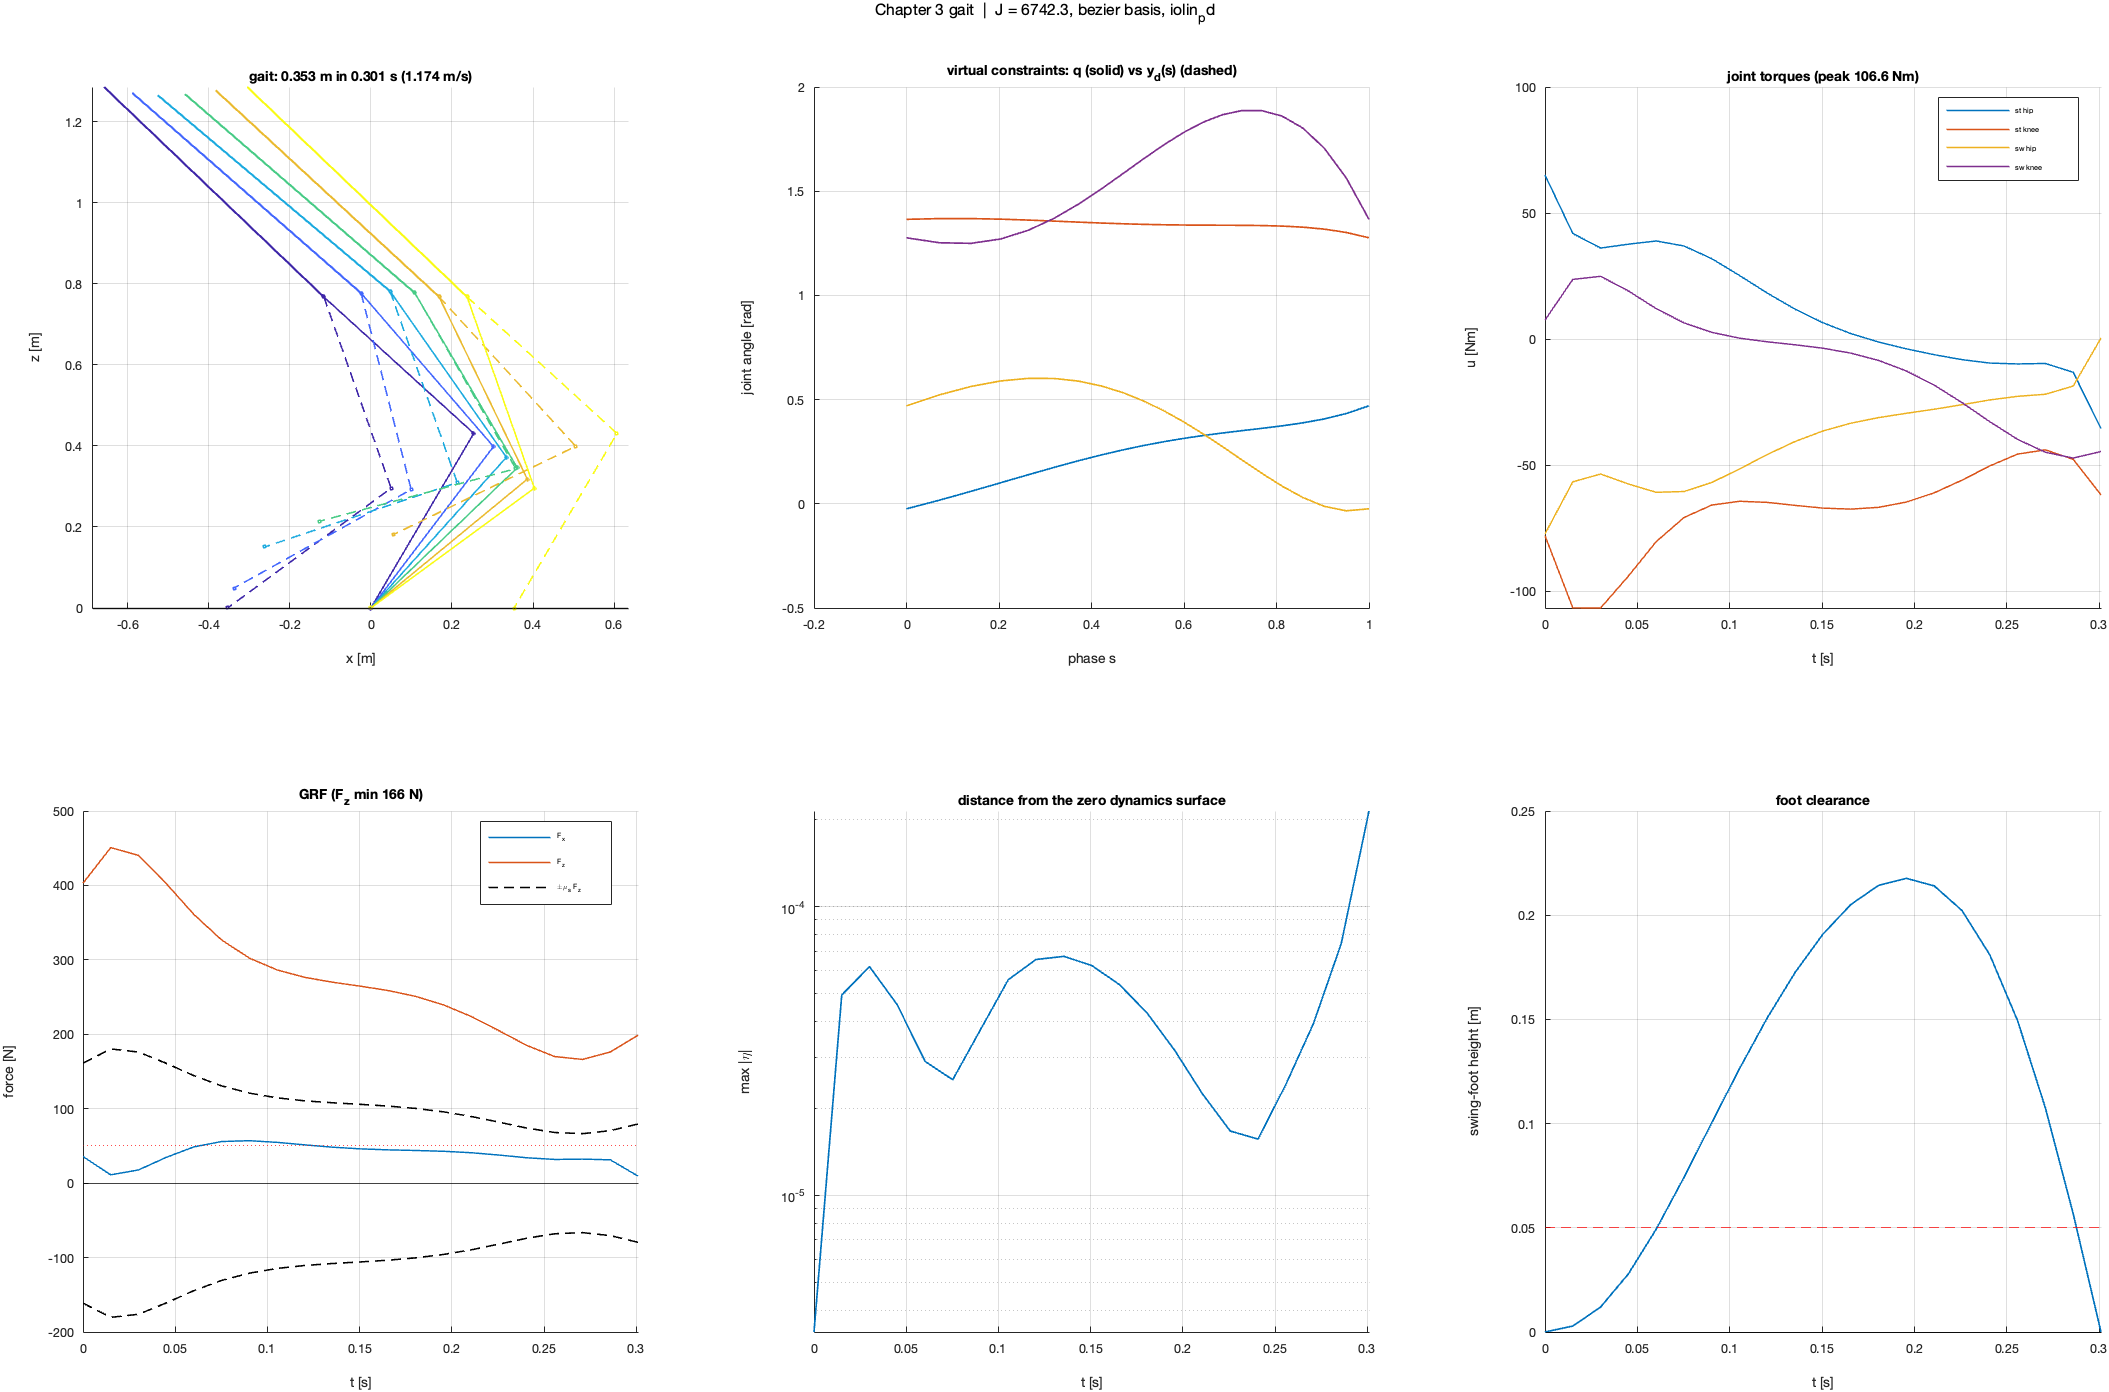
\includegraphics[width=\textwidth]{fig_ch3_reference_gait.png}
\caption{The reference gait, solved on the Bezier basis under
\texttt{iolin\_pd} ($J = 6742.3$). \emph{Top row}: stick-figure snapshots
through one step (solid) against the desired profiles (dashed), 0.353~m in
0.301~s; the virtual constraints $q$ (solid) versus $y_d(s)$ (dashed) in phase;
and the four joint torques, peaking at 106.6~Nm. \emph{Bottom row}: ground
reaction force with the friction cone $\pm\mu_s F_z$ (dashed) and
$F_z^{\min} = 166$~N; the distance $\max|\eta|$ from the zero dynamics surface,
which stays below $10^{-4}$ across the whole step; and swing-foot clearance
against the 0.05~m requirement (dashed). Note that the torque peak reported
here, 106.6~Nm, is taken at the collocation nodes; the 109~Nm in
Table~\ref{tab:gait} is the closed-loop simulated peak.}
\label{fig:gait}
\end{figure*}

Table~\ref{tab:gait} and Fig.~\ref{fig:gait} report the reference gait. It is
periodic, mesh-verified and orbitally stable, and was found with NEC1
\emph{disabled}.

\begin{table}[t]
\caption{Reference gait properties}
\label{tab:gait}
\centering
\begin{tabular}{lc}
\toprule
Quantity & Value \\
\midrule
Walking speed                     & 1.174 m/s \\
Step length / duration            & 0.353 m / 0.301 s \\
Periodicity through $\Delta$      & $8.1\times10^{-7}$ \\
Mesh verification (tol $10^{-3}$) & $6.8\times10^{-4}$ \\
$\max|\eta|$ over nodes           & $2.1\times10^{-4}$ \\
Stance-foot drift                 & $8.7\times10^{-7}$ m \\
Poincar\'e $\rho$                 & \textbf{0.760} (stable) \\
$\delta^2_{\mathrm{zero}}$ (NEC5) & \textbf{0.75996} (stable) \\
$\zeta^*_2$ vs $V_{\max}/\delta^2$ (NEC4) & 3.114 vs 0.601 (holds) \\
NEC3 impulse $|I_x|/I_z$          & \textbf{2.44} vs $\mu_s = 0.4$ (fails) \\
\midrule
Peak torque                       & 109 Nm \\
Impact impulse                    & 12.8 Ns \\
Continuous friction ratio         & 0.194 \\
Minimum normal force              & 166 N \\
\bottomrule
\end{tabular}
\end{table}

Disabling NEC1 was necessary, not merely convenient. Pinning
$L_{\mathrm{step}}/T_{\mathrm{step}} = v_{\mathrm{des}}$ while the gait shape was
still far from periodic over-constrained the problem and the solve stalled on
spurious discrete solutions; releasing it converged to a genuine trajectory
within 120 iterations. Speed is subsequently recovered by continuation rather
than imposed from the start. All four classical Table~3.1 limits are satisfied
\emph{without being enforced}, which is the intended workflow: solve with limits
off, read the measured ranges, then enable them one at a time.

A relevant cautionary note concerns transplanted limits. The thesis limits are
ATRIAS numbers---63~kg with 50:1 harmonic drives, so its ``$|u| \le 5$~Nm'' is
\emph{motor} torque, 250~Nm at the joint. RABBIT is ${\approx}30$~kg and direct
drive, so $u$ \emph{is} joint torque. Copying the numbers across produces an
infeasible problem and a solver that fails in ways that resemble software bugs.

% =====================================================================
\subsection{NEC3 and mesh sensitivity}
\label{sec:nec3}
% =====================================================================

The reference gait fails NEC3: the impact impulse is predominantly
\emph{horizontal} where a walking impact should be predominantly vertical. The
impact map imposes $J_{\mathrm{sw}}\dot q^+ = 0$---the foot sticks---and at
$|I_x|/I_z = 2.44$ against $\mu_s = 0.4$ it would skid instead. The
continuous-phase friction ratio is a comfortable $0.194$, so this violation is
\emph{invisible unless the impulse is checked separately}. This is precisely why
NEC3 is listed apart from NIC2.

NEC3 is also the one constraint in the set that a coarse mesh evaluates
incorrectly (Table~\ref{tab:nec3}).

\begin{table}[t]
\caption{Impulse ratio versus mesh resolution, \texttt{impact} gate \emph{off}}
\label{tab:nec3}
\centering
\begin{tabular}{cccc}
\toprule
Mesh & $|I_x|/I_z$ & $I_z$ [Ns] & Verification \\
\midrule
$N = 21$ & 2.44 & 4.86 & $6.75\times10^{-4}$ (passes) \\
$N = 41$ & 1.35 & 8.34 & $3.57\times10^{-4}$ (passes) \\
\bottomrule
\end{tabular}
\end{table}

Remeshing alone moved the ratio by 80\% with nothing pushing on the impulse. The
$N=21$ gait is not a spurious discrete solution---it passes verification. The
explanation is that mesh verification bounds
$\max|X_{\mathrm{node}} - X_{\mathrm{true}}|$ over the step, whereas the impulse
is $\Lambda(q_N)v_{\mathrm{foot}}(x_N)$ evaluated at a \emph{single endpoint},
with $I_z$ small enough that a $7\times10^{-4}$ state error swamps it. Every
other Table~3.1 quantity is an extremum over the whole step and survives a coarse
mesh; this one does not. The practical consequence is that a constraint ladder
calibrated on the coarse number never becomes active: one attempt starting at
2.20 spent two stages with the constraint inactive while the ratio drifted
\emph{upward}, $1.104 \to 1.261$.

% =====================================================================
\section{Control Law Comparison}
\label{sec:control}
% =====================================================================

Four laws for selecting $\mu$ were implemented: input--output linearizing PD;
a rapidly exponentially stabilizing CLF~\cite{ames2014} solved in closed form;
the unconstrained CLF-QP; and the constrained CLF-QP, which adds the torque box
and, optionally, friction and normal-force limits as linear inequalities---
possible precisely because $\lambda$ is affine in $u$.

Table~\ref{tab:control} reports the same reference gait run under three of these
at 1~kHz with a torque box of 65.5~Nm, deliberately \emph{below} the 109~Nm the
gait requires, so that the constraint genuinely binds.

\begin{table}[t]
\caption{Controllers under a binding 65.5 Nm torque box}
\label{tab:control}
\centering
\begin{tabular}{lcccc}
\toprule
Controller & Peak $|u|$ & Over box & $\max|\eta|$ & $\max\delta$ \\
\midrule
\texttt{iolin\_pd}   & 109.6 & 44.2  & $1.77\times10^{-2}$ & 0 \\
\texttt{clfqp}       & 203.3 & 137.8 & 2.77 & 0 \\
\texttt{clfqp\_con}  & \textbf{65.5} & \textbf{0.0} & 17.4 & 71.5 \\
\bottomrule
\end{tabular}
\end{table}

Only the constrained QP respects the box, and it does so by construction. Two
results deserve emphasis.

\subsection{Minimum-norm is not the same as well-behaved}

The \emph{unconstrained} CLF-QP is the worst of the three. It requests the
least-norm $\mu$ that certifies the required convergence rate at each instant,
and rides that bound at a ratio of exactly $1.0000$. But the RES-CLF inequality
is a \emph{floor} on convergence, not a target, and on this robot the floor is
far too slow: $c_3/\epsilon = 0.732$ is a time constant of 1.37~s against a step
of 0.301~s, so meeting it exactly contracts $V$ by only 20\% per step---while
the impact expands $V$ by up to $34\times$. The hybrid budget is
$0.80 \times 34.1 = 27.3 > 1$, so $\eta$ grows step over step and the demanded
torque nearly doubles.

The surplus convergence that minimum-norm optimization so efficiently eliminates
is exactly what was paying for stability across the impact.

Sampling is not the cause. Measured on the transverse dynamics, varying $dt$
from 1~kHz to 100~Hz gives identical rollouts (peak $|\mu| = 3.0$,
$V(T)/V(0) = 0.802$ at every rate), and $V$ never exceeds its certified
envelope. The continuous-phase guarantee is not violated anywhere---it simply
says nothing about $\Delta$, and the robot is a hybrid system.

\subsection{Slack as an honest signal}

The constrained QP reports $\max\delta = 71.5$. This is the point, not a defect.
The slack variable is the controller announcing that it \emph{could not} meet
the required convergence rate inside the actuator limit; the exponential
guarantee holds only while $\delta = 0$, so this is the theory's boundary being
crossed \emph{visibly}, with $\max|\eta|$ growing to 17.4 as the price. A PD law
has no comparable mechanism: it saturates and voids its guarantee silently.

% =====================================================================
\section{Verification}
% =====================================================================

Each stage is checked against an \emph{independent} reference rather than
against itself: the control-affine split against the raw KKT solve
($1.7\times10^{-13}$); the impact against a hand-built momentum balance
($3.3\times10^{-16}$); Bezier derivatives against finite differences; the
Bezier/B-spline equivalence at matched degree ($1.1\times10^{-16}$);
$\ddot y = L_f^2y + L_gL_fyu$ against the derivative of the \emph{true} flow
($5.1\times10^{-9}$); the closed-form CLF solution against a general-purpose QP
($9.0\times10^{-11}$); the zero-dynamics reduction against the full 14-state
model; and each controller against its \emph{own} Lyapunov certificate.

The suite comprises seven groups and completes in 23.0~s. Six pass. The seventh
is the Hermite--Simpson order assertion of Section~\ref{sec:order}, left failing
deliberately to keep the basis trade-off visible rather than silent.

% =====================================================================
\section{Discussion and Limitations}
% =====================================================================

Three limitations are stated plainly.

The reference gait \textbf{fails NEC3} and is therefore not physically
realizable as an impact without slipping, despite being periodic, stable, and
comfortably within every continuous-phase limit. Correcting it requires marching
the impulse cone down a ladder, because the impulse is a property of one state
filtered through $\Delta$, and that state is pinned by both periodicity and the
guard---the only way to change the impulse is to change the whole orbit.

The shipped configuration \textbf{sacrifices transcription accuracy} for basis
independence, at a measured $4300\times$. This is a defensible choice for a
cross-check but the wrong default for quantitative work.

The stability certificate is \textbf{local}. Both $\rho$ and
$\delta^2_{\mathrm{zero}}$ characterize the linearization about the periodic
orbit; neither bounds the basin of attraction, and the $34\times$ expansion of
$V$ across impact suggests that basin may be small.

% =====================================================================
\section{Conclusion}
% =====================================================================

A complete HZD pipeline for RABBIT was implemented and, more importantly,
measured. The transcription is correct at fifth order, but its \emph{observed}
accuracy is governed by the smoothness of the output basis---a coupling that a
naive mesh-refinement study misattributes to the collocation scheme. Orbital
stability can be certified in closed form from the Bezier coefficients alone,
agreeing with brute-force simulation to five digits at a small fraction of the
cost. And minimum-norm optimality, applied pointwise to a hybrid system,
actively destroys the stability margin it appears to preserve: the constrained
QP is preferable not only because it respects actuator limits but because its
slack variable makes the failure of the guarantee observable.

The single most transferable lesson is methodological. In every case above, the
informative result came from reporting a \emph{distribution} rather than an
extremum---median defect versus maximum defect, impulse ratio versus mesh,
$V$ across the impact versus $V$ within the continuous phase. Aggregate
statistics hid the mechanism; disaggregated ones revealed it.

% =====================================================================
\begin{thebibliography}{1}

\bibitem{westervelt2007}
E.~R. Westervelt, J.~W. Grizzle, C.~Chevallereau, J.~H. Choi, and B.~Morris,
\emph{Feedback Control of Dynamic Bipedal Robot Locomotion}.
Boca Raton, FL: CRC Press, 2007.

\bibitem{chevallereau2003}
C.~Chevallereau \emph{et al.},
``RABBIT: A testbed for advanced control theory,''
\emph{IEEE Control Systems Magazine}, vol.~23, no.~5, pp.~57--79, 2003.

\bibitem{ames2014}
A.~D. Ames, K.~Galloway, K.~Sreenath, and J.~W. Grizzle,
``Rapidly exponentially stabilizing control Lyapunov functions and hybrid zero
dynamics,''
\emph{IEEE Trans. Automatic Control}, vol.~59, no.~4, pp.~876--891, 2014.

\bibitem{hargraves1987}
C.~R. Hargraves and S.~W. Paris,
``Direct trajectory optimization using nonlinear programming and collocation,''
\emph{J. Guidance, Control, and Dynamics}, vol.~10, no.~4, pp.~338--342, 1987.

\bibitem{betts2010}
J.~T. Betts,
\emph{Practical Methods for Optimal Control and Estimation Using Nonlinear
Programming}, 2nd~ed.
Philadelphia, PA: SIAM, 2010.

\bibitem{hereid2017}
A.~Hereid and A.~D. Ames,
``FROST: Fast robot optimization and simulation toolkit,''
in \emph{Proc. IEEE/RSJ Int. Conf. Intelligent Robots and Systems (IROS)}, 2017,
pp.~719--726.

\end{thebibliography}

\end{document}
